

\chapter{La charge électrique}
\section{Introduction}
L'électricité est souvent perçue comme une branche \enquote{moderne} de la physique, elle fait référence aux ampoules, aux machines électriques, à l'électronique et aux méthodes de communications modernes. Toutefois, l'histoire de l'électricité est très ancienne. En effet, les plus anciennes observations connues dans le monde occidental ont été faites par le philosophe grec Thalès de Millet (600 av JC). Puisque Thalès a fait ses découvertes en manipulant de l'ambre jaune (êlektron en grec), il a appelé ce phénomène électricité.



\section{Électricité vitreuse et résineuse}
Si deux tubes en PVC suspendus à un fil, sont frottés avec un tissu, ils se repoussent. De même, si un tube en PVC frotté est approché de petits objets (morceaux de papier, grains de semoule, billes de polystyrène, ...), ceux-ci sont attirés par le tube.
Cette expérience est connue depuis longtemps, mais avant la découverte des matières plastiques, elle se faisait avec de la résine.

\begin{encadre}
    Lorsqu'ils sont frottés, certains corps acquièrent une \motcle{charge électrique}, on dit qu'ils sont électrisés.
\end{encadre}

Si la même manipulation est faite avec un tube en PVC et un tube en verre, ils s'attirent l'un l'autre. Ceci permet de mettre en évidence l'existence de deux types de charges électriques, autrefois appelées électricité vitreuse et électricité résineuse, mais plus simplement nommées \motcle{charges positives} et \motcle{charges négatives} depuis les travaux de Benjamin Franklin. Il a associé de manière complètement arbitraire l'électricité positive à l'électricité vitreuse. Cette convention est encore utilisée de nos jours et a comme conséquence la notion de \motcle{sens réel} et \motcle{sens conventionnel} du courant électrique (voir encadré).

\begin{figure}[!ht]
    \centering
    \begin{minipage}[b]{.47\linewidth}
        \centering
        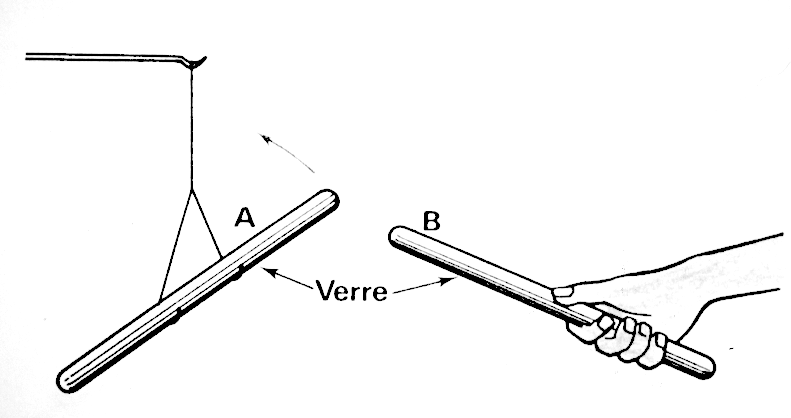
\includegraphics[width=.8\linewidth]{verre_verre.png}
        \caption{Deux tiges en verre électrisées}
        \label{verre_verre}
    \end{minipage}
    \begin{minipage}[b]{.47\linewidth}
        \centering
        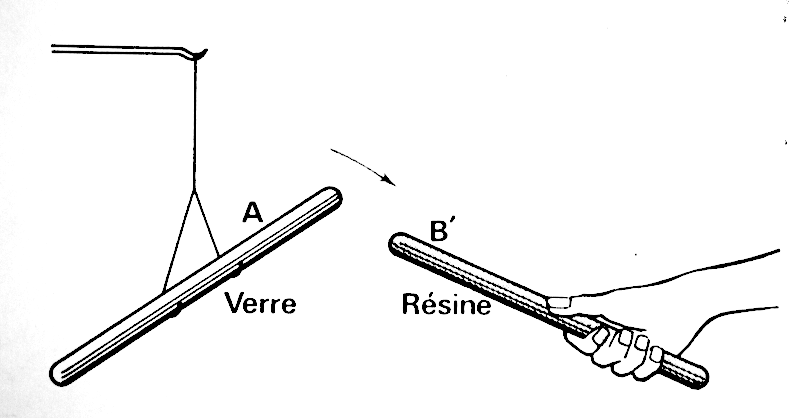
\includegraphics[width=.8\linewidth]{verre_resine.png}
        \caption{Une tige en verre et une tige en résine électrisées}
        \label{verre_resine}
    \end{minipage}
\end{figure}

\subsection{Conservation de la charge}
Lorsqu'on frotte des objets pour les électriser, des électrons sont arrachés par l'un et s'accumulent sur l'autre. Il n'y a donc pas réellement de création de charge, plutôt une répartition de celles-ci. C'est un exemple de la loi de conservation de la charge électrique.
\begin{encadre}
    La quantité nette de charge électrique produite au cours de n'importe quelle transformation est nulle.
\end{encadre}

\newpage

\subsection{La charge électrique}
La \enquote{quantité d'électricité} qui peut s'accumuler localement se mesure à l'aide de la charge électrique.
\begin{encadre}
    \motcle{charge électrique} : q [Coulomb ; C]
\end{encadre}
Concrètement, les charges apparaissent sous l'effet de déplacement d'électrons ou de protons. La charge d'un électron est de : \(q=- 1,6 \times 10^{-19}[C]\)

\section{Isolants, conducteurs et résistance}
Puisque les charges de mêmes signes se repoussent et que celles de signes contraires s'attirent, les particules chargées peuvent bouger. Elles ne le font cependant pas avec la même facilité dans tous les matériaux. Ceux dans lesquels les charges se déplacent facilement sont appelés \motcle{conducteurs}tandis que ceux dans lesquels les charges se déplacent difficilement et qui empêchent dés lors le passage de l'électricité sont appelés \motcle{isolants}. Le pouvoir isolant d'un corps est mesuré par sa résistance électrique.

\begin{encadre}
    \motcle{résistance électrique} : R [Ohm ; \(\Omega\)]
\end{encadre}

\newpage
\begin{tcolorbox}[colback=mygray1,breakable,colframe=mygray2,sharp corners=northwest,title=Sens conventionnel et sens réel du courant électrique]

    C'est le Français Charles-François de Cisternay Dufay (1698-1739) qui, en frottant du verre et de l'ambre, constate la différence de comportement électrique de ces deux corps. Chacun repoussant ce qui a été mis en contact avec lui même (le verre) et attirant ce qui a été mis en contact avec l'autre (l'ambre).
    Il en déduit l'existence de deux espèces d'électricité qu'il nomme \enquote{vitrée} et \enquote{résineuse} et énonce la loi d'attraction et de répulsion:
    \enquote{Deux corps portant la même espèce d'électricité se repoussent, deux corps portant des électricités différentes s'attirent.}

    L'Américain Franklin (1706-1790), abordant l'électricité en autodidacte, imagine l'électricité comme un fluide unique qui imprègne tous les corps.
    Le frottement fait simplement passer ce fluide d'un corps dans l'autre. Le corps qui en a reçu est alors chargé positivement, celui qui en a perdu l'étant négativement.
    Ainsi, propose Franklin, le verre frotté prend de l'électricité au corps qui le frotte. Il se charge \enquote{positivement} alors que le soufre ou l'ambre, qui perdent de l'électricité par frottement, se chargent \enquote{négativement}.
    La théorie des deux fluides s'impose en Europe continentale. Celle du fluide unique de Franklin conserve la faveur des britanniques.
    Tant qu'il ne s'agit que d'étudier les propriétés statiques de l'électricité, cette divergence ne prête pas à conséquence. Le problème devient plus épineux après 1800 et la découverte de la pile électrique par Volta.
    En effet cette pile produit, en continu, un \enquote{courant} d'électricité. La question se pose donc : quel est son sens dans un circuit extérieur ?
    Pour les partisans de Franklin, aucun problème : la pile ne fournit qu'une seule espèce d'électricité. Le courant circule donc nécessairement du pôle qui porte le plus, le pôle positif, vers celui qui en porte le moins, le pôle négatif.
    Pas de problème non plus pour les partisans de Dufay qui ont une explication : la pile produit les deux espèces d'électricité. Dans le conducteur il existe deux courants. Le courant de fluide positif circule du pôle + au pôle -, celui d'électricité négative du pôle - au pôle +.
    Comme la théorie des deux espèces d'électricité, celle des deux courants s'impose dans l'Europe continentale. Celle du courant unique chez les britanniques.
    C'est au moment où, en 1820, Oersted découvre l'effet magnétique des courants qu'une convention est proposée par Ampère, lui même partisan des deux courants.

    On conviendra dit-il, d'appeler \motcle{sens du courant} , celui dans lequel circule le fluide positif et on se souviendra, dit-il, que le fluide négatif circule en sens contraire. Par cette convention, partisans de Franklin et de Dufay se rencontrent à nouveau. Pour les uns le sens \enquote{conventionnel} est le sens réel de circulation du fluide unique. Pour les autres, ce sens est uniquement celui de circulation du fluide positif.
    La découverte de l'électron par Thomson et Perrin en 1897, puis celle de la structure de l'atome, révèle l'erreur initiale de Franklin : le verre ne gagne pas d'électricité dans le frottement, il en perd ! Il faut donc attribuer une charge négative à ces porteurs d'électricité que sont les particules que l'on désignera ensuite par le terme d'électrons.

    Par ailleurs, les partisans de Dufay et des deux courants ne peuvent pas, eux non plus, triompher. Il existe bien deux espèces d'électricité, mais dans un conducteur métallique seul un fluide circule. L'électricité positive portée par les noyaux des atomes est fixe. Seule l'électricité négative portée par les électrons peut circuler.

    Ainsi il existe bien un seul courant, mais, constitué d'électrons, il circule dans le sens inverse du sens conventionnel !

    Pourquoi ne pas changer les conventions concernant le signe des charges et le sens du courant? En 1900, l'industrie de l'électricité construite sur les conventions du début du siècle s'est développée. Aucune tentative ne sera faite pour inverser le sens du courant conventionnel. Les signes + et - des charges, ainsi que le sens du courant ne sont, depuis, plus que des conventions mathématiques.\footnote{Cette section est basée sur un article paru dans le \enquote{Bulletin de l'Union des Physiciens},Vol. 88, janvier 1994}

\end{tcolorbox}
